\section{Architettura del sistema}
Lo scopo dell'applicazione \textbf{ADCrm} è quello di rispondere alle richieste provenienti da ADProject, recuperando in tempo reale i dati desiderati dal CRM ed elaborarli per renderli fruibili.\\
Per supplire a questa necessità, ADCrm presenta un'architettura client-server, assumendone entrambi i ruoli:
\paragraph{Server}
L'applicazione assume il ruolo di server nel momento in cui deve assolvere alle richieste provenienti da ADProject mediante le \glo{API} REST. Deve quindi rispondere a due esigenze principali:
\begin{itemize}
	\item esporre \glo{API} REST per poter rispondere, in formato \glo{JSON}, alle richieste \gls{http} ricevute;
	\item salvare i dati, non sensibili, necessari per il processo di autenticazione e collegamento con il CRM su un piccolo database interno.
\end{itemize} 

Si è deciso di mantenere il database sul servizio ADCrm per togliere l'onere ad ADProject di conoscere: non solo le procedure di autenticazione al CRM, ma anche la tipologia di CRM che si va ad interrogare (Salesforce, Dynamics, ...). In questo modo si riesce a mantenere una netta separazione dei ruoli tra le varie componenti. 

\paragraph{Client}
L'applicazione assume il ruolo di client nel momento in cui deve interrogare il server del CRM per recuperare i dati di cui ha bisogno ADProject, deve quindi:
\begin{itemize}
	\item interrogare il server remoto attraverso il set di \glo{API} esposto;
	\item organizzare i dati ricevuti in modo tale che siano fruibili da ADProject;
	\item restituire gli stessi in formato \glo{JSON}.
\end{itemize}

Nelle prime fasi della progettazione si è valutata l'ipotesi di utilizzare un database per fare \glo{caching} dei dati provenienti dal CRM, così da limitare le richieste \gls{http} necessarie e da velocizzare le risposte fornite, tuttavia la necessità di ADProject di utilizzare sempre dati aggiornati ha fatto abbandonare quest'opzione.\\

La figura \ref{fig:architetturasistema} illustra l'architettura ad alto livello del sistema; una descrizione più dettagliata delle varie componenti verrà esposta nelle sezioni successive.

\begin{figure}[H]
	\centering
	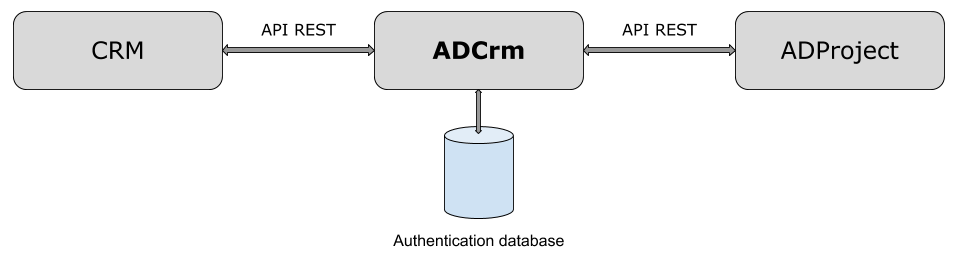
\includegraphics[width=\linewidth]{images/architettura_sistema}
	\caption{Architettura ad alto livello}
	\label{fig:architetturasistema}
\end{figure}

\section{API REST}\label{apiRest}
Di seguito si trova la definizione delle \glo{API} REST esposte dal servizio ADCrm.\\
I metodi \gls{http} con cui chiamare tutti i successivi URL sono metodi \textbf{GET} ed i dati ricevuti nelle risposte sono forniti in formato \glo{JSON}.

	\begin{small}
		\begin{longtable}{ | l | p{8cm} | }
			\hline \textbf{URL} & \textbf{Descrizione Risposta}\\
			\hline api/organization/\{organizationId\}/ & Risponde con i dati riguardante l'organizzazione avente \textit{id = organizationId}\\
			\hline
		\end{longtable}		
	\end{small}
Questo primo \glo{endpoint} necessita di ulteriori spiegazioni in quanto l'url specificato sopra è da anteporre a di tutti quelli che seguiranno \\(eg. "\textbf{api/organization/\{organizationId\}/accounts}" nel caso dell'url "/accounts").\\
Inoltre si noti che è necessario da parte di chi effettua chiamate verso questo url (e quindi anche verso tutti gli altri) conoscere il campo \textit{organizationId} per poter ottenere una risposta. Questa restrizione è stata posta per far si che il sistema sia più sicuro, rendendo disponibili dei dati riguardanti l'azienda fruitrice del servizio solo se si conosce il corretto identificativo.
%TODO: decidere se sistemare la parte qua sopra
	\begin{small}
		\begin{longtable}{ | l | p{8cm} | }
			\hline \textbf{URL} & \textbf{Descrizione Risposta}\\
			\hline /accounts & Risponde con la lista contenente i dati di tutti gli account\\
			\hline /accounts/\{\textit{accountId}\} & Risponde con i dati dell'account avente \textit{id = accountId}\\    
			\hline /accounts/\{\textit{accountId}\}/contacts & Risponde con la lista contenente i dati di tutti gli i contatti legati all'account avente \textit{id = accountId}\\
			\hline /accounts/\{\textit{accountId}\}/proposals & Risponde con la lista contenente i dati di tutte le offerte commerciali legate all'account avente \textit{id = accountId}\\
			\hline /contacts/\{\textit{contactId}\} & Risponde con i dati del contatto avente \textit{id = contactId}\\
			\hline /proposals & Risponde con la lista contenente i dati di tutte le proposte commerciali\\
			\hline /proposals/\{\textit{proposalId}\} & Risponde con i dati della proposta commerciale avente \textit{id = proposalId}\\    
			\hline /proposals/\{\textit{proposalId}\}/products & Risponde con una lista contenente tutti i prodotti legati all'offerta commerciale avente \textit{id =  proposalId}\\
			\hline /products/\{\textit{productId}\} & Risponde con i dati del prodotto avente \textit{id = productId}\\
			\hline /users & Risponde con una lista contenente i dati di tutti gli utenti del CRM\\
			\hline /users/\{\textit{userId}\} & Risponde con i dati del utente avente \textit{id = userId}\\    
			\hline /productCategories & Risponde con una lista contenente i dati di tutte le famiglie di prodotti\\
			\hline /productCategories/\{\textit{categoryId}\} & Risponde con i dati della famiglia di prodotti avente \textit{id = categoryId}\\		
			\hline 
		\end{longtable}		
	\end{small}
	
\section{Progettazione}
In questa sezione verranno descritti in maniera dettagliata tutti i \glo{package}, le classi principali dell'applicazione e i metodi più importanti delle stesse al fine mostrare al meglio il progetto di stage svolto.

%\begin{figure}[H]
%	\centering
%	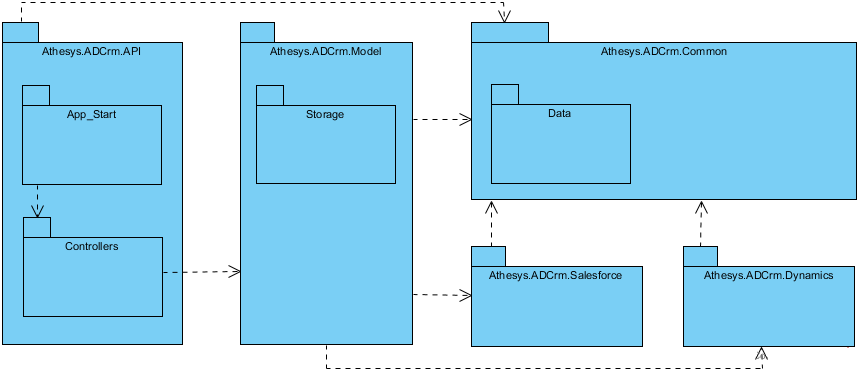
\includegraphics[width=\linewidth]{images/modulesDiagram}
%	\caption{Diagramma dei moduli di ADCrm}
%	\label{fig:generalUMLDiagram}
%\end{figure}

\begin{figure}[H]
	\centering
	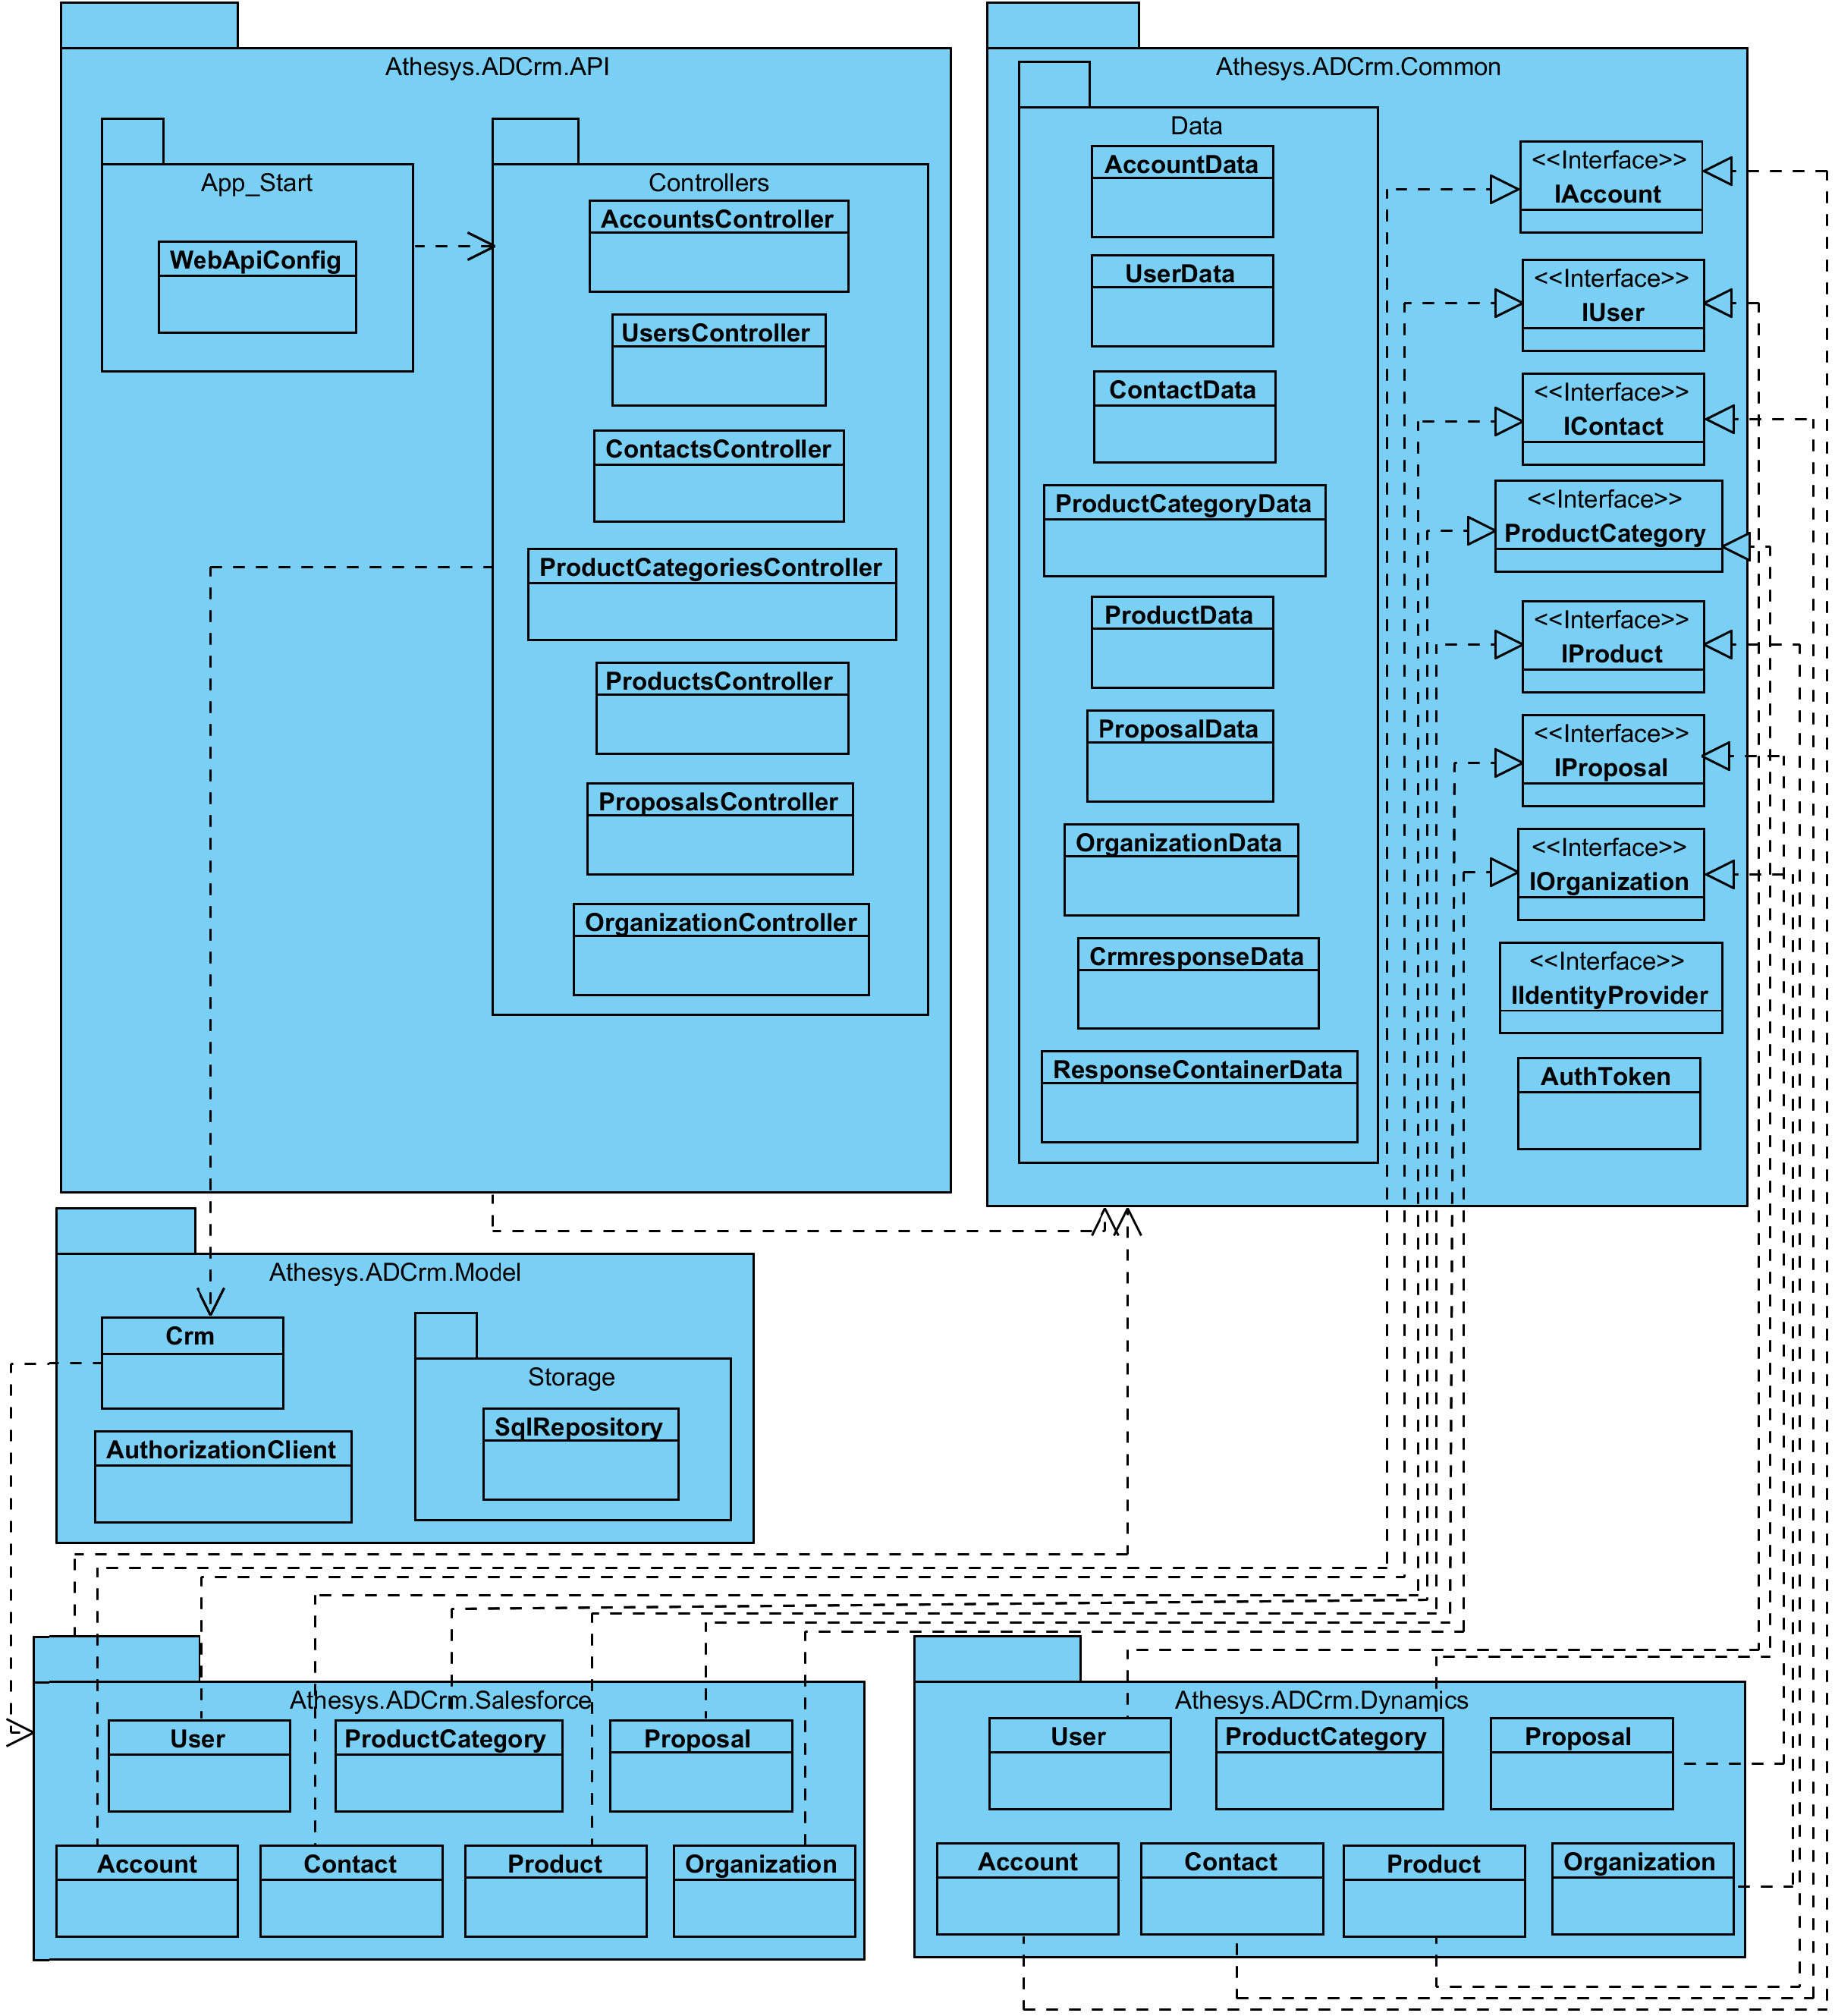
\includegraphics[width=\linewidth]{images/general2}
	\caption{Diagramma UML di ADCrm}
	\label{fig:modulesdiagram}
\end{figure}
\newpage
Nella figura \ref{fig:modulesdiagram} viene illustrato il diagramma \glo{UML} delle classi dell'applicazione.

\subsection{Athesys.ADCrm.API}
\begin{figure}[H]
	\centering
	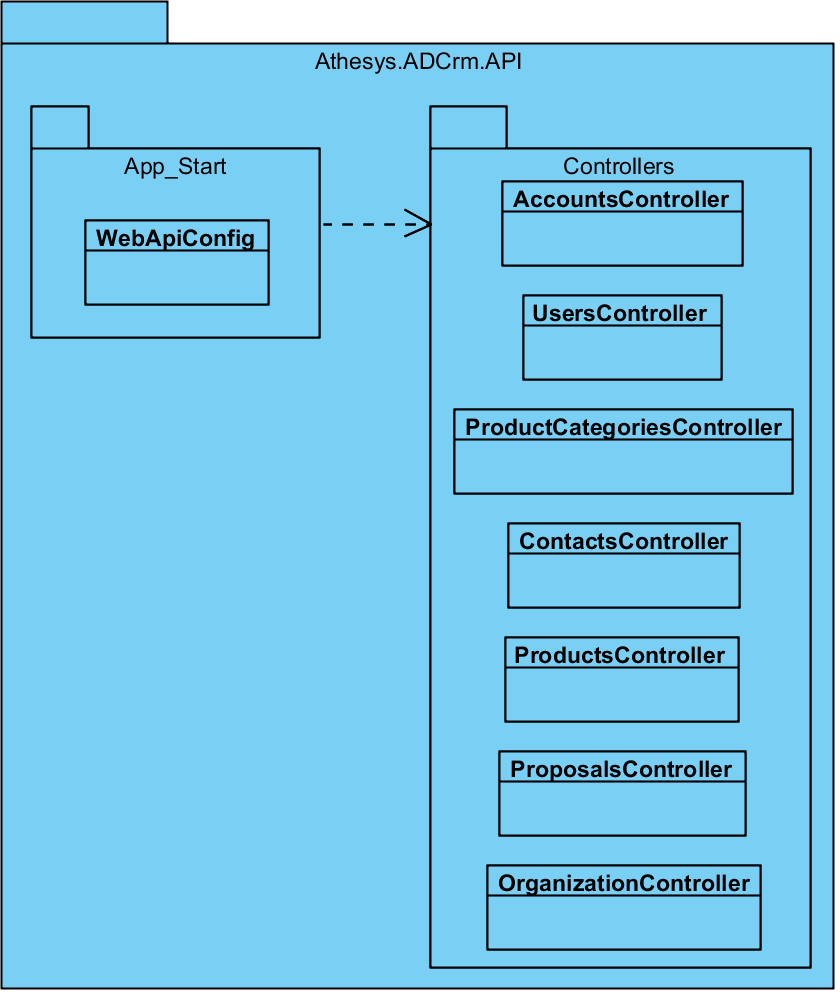
\includegraphics[width=\linewidth]{images/modules/API}
	\caption{Diagramma UML del package Athesys.ADCrm.API}
	\label{fig:api}
\end{figure}
\paragraph{Descrizione:} 
Questo \glo{package} è utilizzato per esporre le \glo{API} REST all'applicazione web ADProject. In esso vengono definite le \glo{route} che è possibile chiamare, ad ognuna di esse viene associato un metodo di un particolare controller. 





\subsection{Athesys.ADCrm.API.AppStart}
\paragraph{Descrizione:} 
Questo \glo{package} contiene la classe che si occupa di definire le \glo{route} che verranno esposte dall'applicazione.
\vfill
\subsection{Athesys.ADCrm.API.Controllers}
\begin{figure}[H]
	\centering
	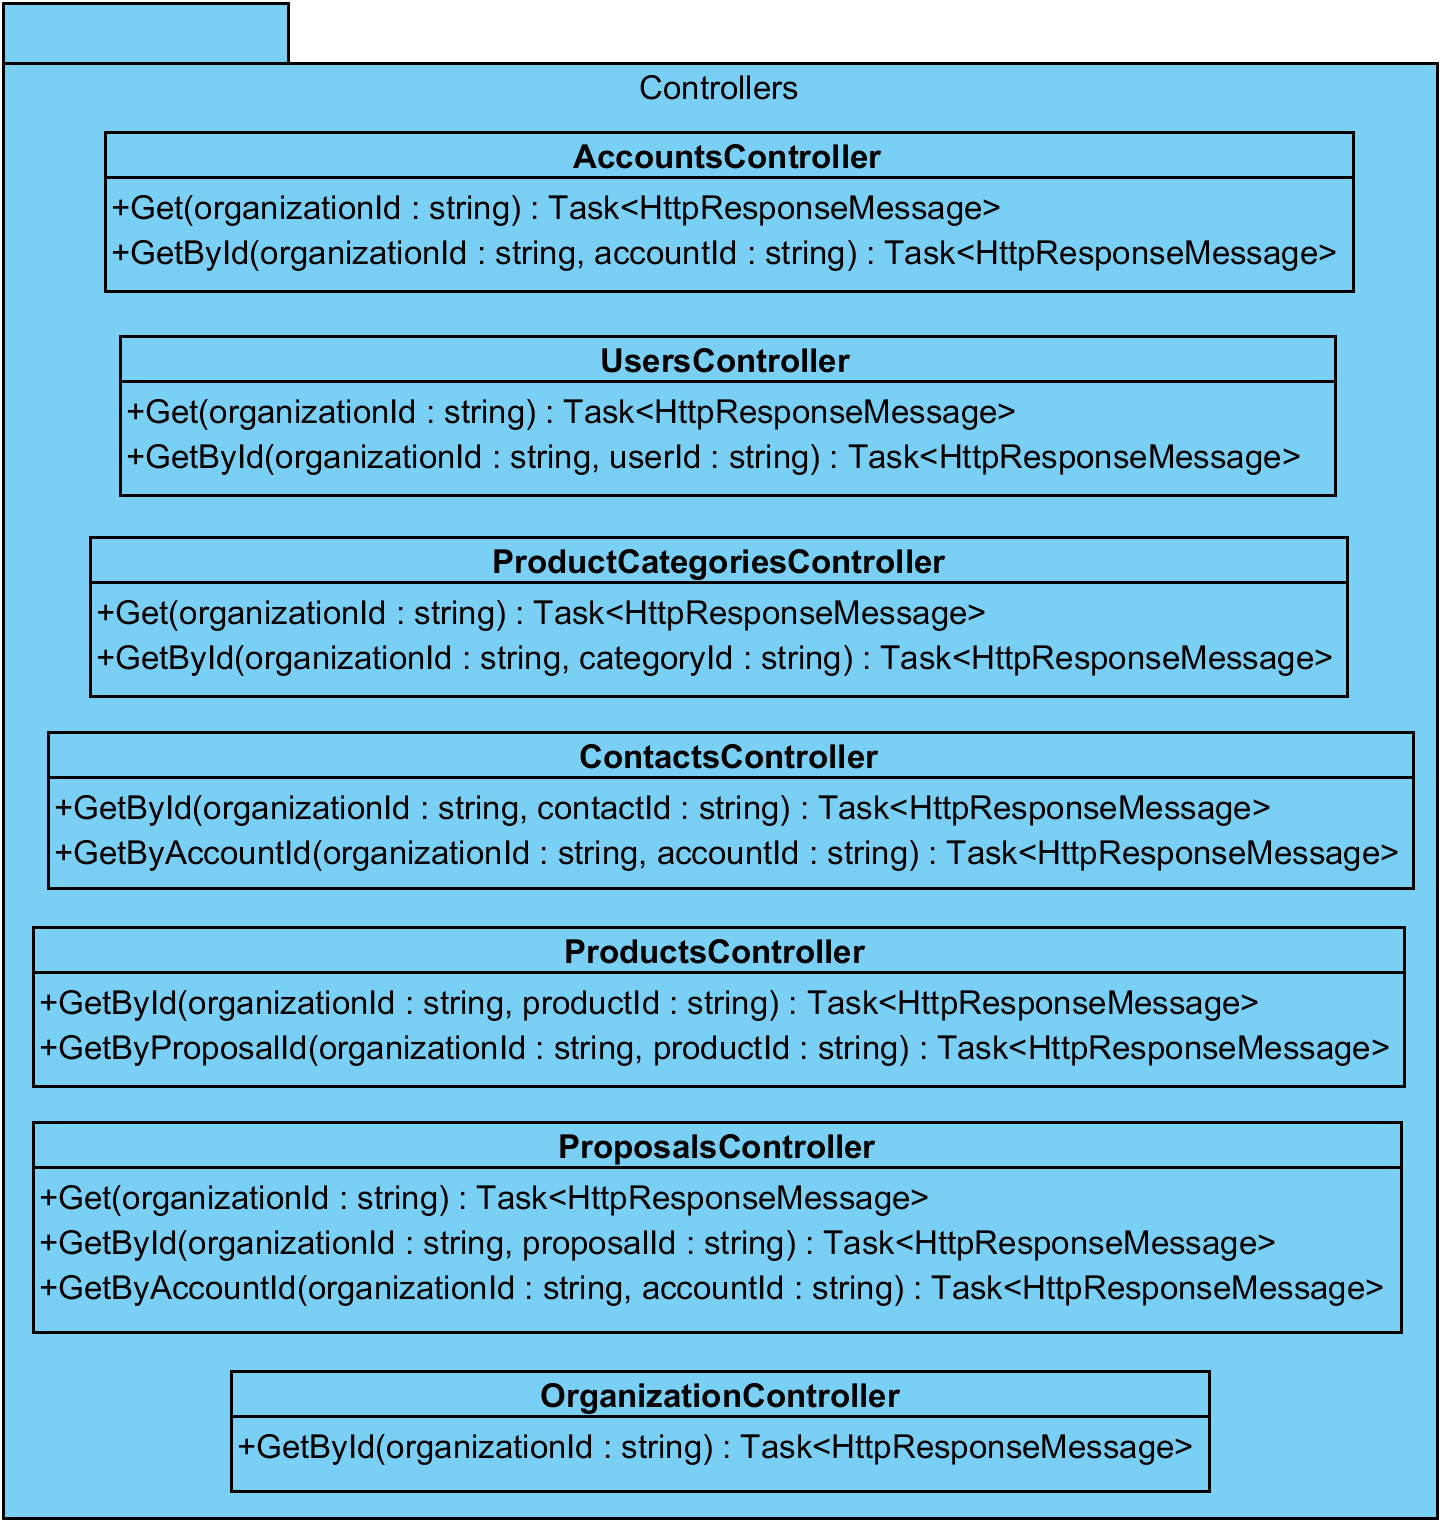
\includegraphics[width=\linewidth]{images/modules/Controllers}
	\caption{Diagramma UML del package Athesys.ADCrm.API::Controllers}
	\label{fig:controllers}
\end{figure}
\paragraph{Descrizione:} Questo \glo{package} contiene tutte le classi controller contenenti i metodi necessari a rispondere alle richieste \gls{http} effettuate alle \glo{route}.


\subsubsection{AccountsController (class)} \label{accountsController}
\paragraph{Descrizione:}
Classe che serve per gestire le chiamate \gls{http} richiedenti dati relativi all'entità Account. Utilizzando la classe Athesys.ADCrm.Model::Crm (che implementa il design pattern Factory) vengono creati oggetti sui quali si possono invocare metodi per interrogare le \glo{API} di uno specifico CRM.
I dati recuperati vengono incapsulati in una risposta \gls{http} e ritornati ad ADProject.

\paragraph{Metodi:}\hfill
\begin{itemize}
	\itemsep0em 
	\item 
		\begin{lstlisting}
		Public async Task<HttpResponseMessage> Get(organizationId : string)
		\end{lstlisting}
		Metodo invocato quando viene inviata una richiesta \gls{http} GET alla route "api/organization/{organizationId}/accounts", ritornado una risposta \gls{http} contenente la lista di tutti gli Account censiti nel CRM.\\
		\textbf{\small Argomenti:}
		\begin{enumerate}[leftmargin=*]
			\itemsep0em 
			\item \begin{lstlisting}
			organizationId : string 
			\end{lstlisting}
			Rapprensenta l'identificativo univoco legato all'utenza aziendale con cui accedere al servizio CRM
		\end{enumerate}
		
	\item 
		\begin{lstlisting}
		Public async Task<HttpResponseMessage> GetById(organizationId : string, accountId : string)
		\end{lstlisting}
		Metodo invocato quando viene inviata una richiesta \gls{http} GET alla route "api/organization/{organizationId}/accounts/{accountId}", ritornando una risposta \gls{http} contenente l'Account avente id = {accountId}.\\
		\textbf{\small Argomenti:}
		\begin{enumerate}[leftmargin=*]
			\itemsep0em 
			\item 
				\begin{lstlisting}
				organizationId : string 
				\end{lstlisting}
				Rappresenta l'identificativo univoco legato all'utenza aziendale con cui accedere al servizio CRM
			\item 
				\begin{lstlisting}
				accountId : string
				\end{lstlisting}
				Rappresenta l'identificativo univoco legato ad un Account del CRM, attraverso il quale si andrà a richiedere i dati voluti
		\end{enumerate}
\end{itemize}

\subsubsection{ProposalsController (class)}

\paragraph{Descrizione:}
Classe che serve per gestire le chiamate \gls{http} richiedenti dati relativi all'entità Proposal. Utilizzando la classe Athesys.ADCrm.Model::Crm (che implementa il design pattern Factory) vengono creati oggetti sui quali si possono invocare metodi per interrogare le \glo{API} di uno specifico CRM. I dati recuperati vengono incapsulati in una risposta \gls{http} e ritornati ad ADProject.

\paragraph{Metodi:}\hfill
\begin{itemize}
	\itemsep0em 
	\item 
	\begin{lstlisting}
	Public async Task<HttpResponseMessage> Get(organizationId : string)
	\end{lstlisting}
	Metodo invocato quando viene inviata una richiesta \gls{http} GET alla route "api/organization/{organizationId}/proposals", ritornando una risposta \gls{http} contenente tutte le offerte commerciali censite nel CRM.\\
	\textbf{\small Argomenti:}
	\begin{enumerate}[leftmargin=*]
		\itemsep0em 
		\item \begin{lstlisting}
		organizationId : string 
		\end{lstlisting}
		Rappresenta l'identificativo univoco legato all'utenza aziendale con cui accedere al servizio CRM.
	\end{enumerate}
	
	\item 
	\begin{lstlisting}
	Public async Task<HttpResponseMessage> GetById(organizationId : string,  proposalId : string)
	\end{lstlisting}
	Metodo invocato quando viene inviata una richiesta \gls{http} GET alla route "api/organization/{organizationId}/proposals/{proposalId}", ritornando una risposta \gls{http} contenente l'offerta commerciale avente id = {proposalId}.\\
	\textbf{\small Argomenti:}
	\begin{enumerate}[leftmargin=*]
		\itemsep0em 
		\item 
		\begin{lstlisting}
		organizationId : string 
		\end{lstlisting}
		Rapprensenta l'identificativo univoco legato all'utenza aziendale con cui accedere al servizio CRM;
		\item 
		\begin{lstlisting}
		proposalId : string
		\end{lstlisting}
		Rappresenta l'identificativo univoco legato ad un offerta commerciale del CRM, attraverso il quale si andrà a richiedere i dati voluti.
	\end{enumerate}

	\item 
	\begin{lstlisting}
	Public async Task<HttpResponseMessage> GetByAccountId(organizationId : string,  accountId : string)
	\end{lstlisting}
	Metodo invocato quando viene inviata una richiesta \gls{http} GET alla route "api/organization/{organizationId}/accounts/{accountId}/proposals", ritornando una risposta \gls{http} contenente la lista delle proposte legate all'account avente id = {proposalId}.\\
	\textbf{\small Argomenti:}
	\begin{enumerate}[leftmargin=*]
		\itemsep0em 
		\item 
		\begin{lstlisting}
		organizationId : string 
		\end{lstlisting}
		Rapprensenta l'identificativo univoco legato all'utenza aziendale con cui accedere al servizio CRM;
		\item 
		\begin{lstlisting}
		accountId : string
		\end{lstlisting}
		Rappresenta l'identificativo univoco legato all'account di un azienda cliente CRM, attraverso il quale si andrà a richiedere i dati voluti.
	\end{enumerate}
\end{itemize}

\vfill
\subsection{Athesys.ADCrm.Common}

	\begin{figure}[H]
		\centering
		\rotatebox{90}{\includegraphics[width=.89\textheight,height=1.08\linewidth]{images/modules/common}}
		
		\caption{Diagramma UML del package Athesys.ADCrm.Common}
		\label{fig:common}
	\end{figure}


\newpage
\paragraph{Descrizione:}
Questo \glo{package} contiene il \glo{package} Data(avente le classi \gls{DTO}) e tutte le interfacce che dovranno essere implementate diversamente per ogni CRM che si vuole collegare all'applicazione. 
%TODO: da modificare la descrizione

\subsubsection{IIdentityProvider (interface)}

\paragraph{Descrizione:}
Interfaccia che dovrà essere implementata dalle classi concrete Athesys.ADCrm.Salesforce::IdentityProvider e\\ Athesys.ADCrm.Dynamics::IdentityProvider, essa definisce i metodi utilizzati per ottenere i \glo{token} di autenticazione e di refresh dai CRM, ed inoltre espone il metodo per effettuare inviare le \glo{query} di recupero dei dati.

\paragraph{Metodi:}\hfill
\begin{itemize}
	\itemsep0em 	
	\item 
	\begin{lstlisting}
	 Task<AuthToken> GetAuthTokenAsync(string authorizationCode, string clientId, string clientSecret, string redirectUrl)
	\end{lstlisting}
	Metodo da implementare per ottenere i \glo{token} da aggiungere all'\glo{header} delle richieste \gls{http} per poter effettuare le query al CRM e il \glo{token} di refresh per otterene nuovi \glo{token} una volta scaduti. Tutti i paramentri passati al metodo sono essenziali per effettuare la suddetta richiesta.\\
	\textbf{\small Argomenti:}
	\begin{enumerate}[leftmargin=*]
		\itemsep0em 
		\item 
		\begin{lstlisting}
		authorizationCode : string
		\end{lstlisting}
		E' un codice che viene generato nel caso l'utente abbia inserito le credenziali d'accesso al CRM;
		%TODO: da aggiungere i riferimenti alla sezione;
		\item 
		\begin{lstlisting}
		clientSecret : string
		\end{lstlisting}
		E' un codice alfanumerico identificativo dell'applicazione, che non cambia nel tempo, generato dall'CRM. Esso è fondamentale per permettere il collegamento OAuth all'applicazione; 
		%TODO: in caso da modificare questa parte
		\item 
		\begin{lstlisting}
		clientId : string
		\end{lstlisting}
		E' un codice alfanumerico che non cambia nel tempo, generato dall'CRM. Esso è fondamentale per permettere il collegamento Oauth all'applicazione. 
		%TODO: in caso da modificare questa parte
		\item 
		\begin{lstlisting}
		redirectUrl : string
		\end{lstlisting}
		E' l'url su cui si vuole far arrivare le risposte del CRM.
		%TODO: in caso da modificare questa parte
	\end{enumerate}
	
	\item 
	\begin{lstlisting}
	Task<string> RenewAuthTokenAsync(string refreshToken, string clientId, string clientSecret)
	\end{lstlisting}
	Metodo da implementare per ottenere un nuovo \glo{token} di autorizzazione nel caso il precedente sia scaduto.\\
	\textbf{\small Argomenti:}
	\begin{enumerate}[leftmargin=*]
		\itemsep0em
		\item 
		\begin{lstlisting}
		refreshToken : string
		\end{lstlisting}
		E' un codice generato dall'CRM fornito una volta effettuato l'accesso con OAuth. Questo permette di ottenere nuovi \glo{token} di autorizzazione senza dover effettuare nuovamente la procedura di login;
		\item 
		\begin{lstlisting}
		clientId : string
		\end{lstlisting}
		E' un codice alfanumerico che non cambia nel tempo, generato dall'CRM. Esso è fondamentale per permettere il collegamento OAuth all'applicazione. 
		%TODO: in caso da modificare questa parte
		\item 
		\begin{lstlisting}
		clientSecret : string
		\end{lstlisting}
		E' un codice alfanumerico identificativo dell'applicazione, che non cambia nel tempo, generato dall'CRM. Esso è fondamentale per permettere il collegamento OAuth all'applicazione; 
		%TODO: in caso da modificare questa parte
	\end{enumerate}

	\item 
	\begin{lstlisting}
	 public async Task<QueryResponse> SendQueryWithRefresh(string resourceProvider,string accessToken,string refreshToken,string clientId, string clientSecret, Action<HttpRequestMessage> addQuryAction)
	\end{lstlisting}
	Metodo da implementare per inviare la richiesta \gls{http} con la \glo{query} per ottenere i dati desiderati dal CRM. Nel caso il \glo{token} d'autorizzazione passato fosse scaduto il metodo si occupa di recuperarne uno nuovo tramite la procedura di refresh. Nella successiva descrizione degli argomenti, per evitare inutili ripetizioni, vengono esclusi quelli già descritti nei sopracitati metodi.\\
	\textbf{\small Argomenti:}
	\begin{enumerate}[leftmargin=*]
		\itemsep0em
		\item 
		\begin{lstlisting}
		resourceProvider : string
		\end{lstlisting}
		E' l'\glo{URI} a cui si devono effettuare le \glo{query};
		\item 
		\begin{lstlisting}
		addQuryAction : Action<HttpRequestMessage>
		\end{lstlisting}
		E' il corpo della \glo{query} in formato di HttpRequestMessage. 
		%TODO: in caso da modificare questa parte
	\end{enumerate}
\end{itemize}

\subsubsection{IProposal (interface)}

\paragraph{Descrizione:}
Interfaccia che dovrà essere implementata dalle classi concrete Athesys.ADCrm.Salesforce::Proposal e\\ Athesys.ADCrm.Dynamics::Proposal, essa definisce i metodi utilizzati per interrogare i rispettivi CRM attraverso le \glo{API} REST esposte, restituendo la risposta \gls{http} incapsulata all'interno di un \gls{DTO} di tipo ResponseContainerData.

\paragraph{Metodi:}\hfill
\begin{itemize}
	\itemsep0em 
	\item 
	\begin{lstlisting}
	Task<ResponseContainerData<ProposalData>> GetAll()
	\end{lstlisting}
	Metodo da implementare per interrogare il CRM ritornando la lista di tutte le offerte commerciali censite nello stesso. Il metodo restituisce il \gls{DTO} ResponseContainerData istanziato al tipo ProposalData essendo una classe \glo{generic}.\\
	
	\item 
	\begin{lstlisting}
	Task<ResponseContainerData<ProposalData>> GetById(proposalId : string)
	\end{lstlisting}
	Metodo da implementare per interrogare il CRM ritornando l'offerta commerciale avente id = {proposalId}. Il metodo restituisce il \gls{DTO} ResponseContainerData istanziato al tipo ProposalData essendo una classe \glo{generic}.\\
	\textbf{\small Argomenti:}
	\begin{enumerate}[leftmargin=*]
		\itemsep0em 
		\item 
		\begin{lstlisting}
		proposalId : string
		\end{lstlisting}
		Rappresenta l'identificativo univoco legato ad un offerta commerciale del CRM, attraverso il quale si andrà a richiedere i dati voluti.
	\end{enumerate}
	
	\item 
	\begin{lstlisting}
	Task<ResponseContainerData<ProposalData>> GetByAccountId(accountId : string)
	\end{lstlisting}
	Metodo da implementare per interrogare il CRM ritornando la lista di tutte le offerte commerciali legate all'account avente id = {accountId}. Il metodo restituisce il \gls{DTO} ResponseContainerData istanziato al tipo ProposalData essendo una classe \glo{generic}.\\
	\textbf{\small Argomenti:}
	\begin{enumerate}[leftmargin=*]
		\itemsep0em
		\item 
		\begin{lstlisting}
		accountId : string
		\end{lstlisting}
		Rappresenta l'identificativo univoco legato all'account di un azienda cliente CRM, attraverso il quale si andrà a richiedere i dati voluti.
	\end{enumerate}
\end{itemize}
\vfill
\subsection{Athesys.ADCrm.API.Data}
\begin{figure}[H]
	\centering
	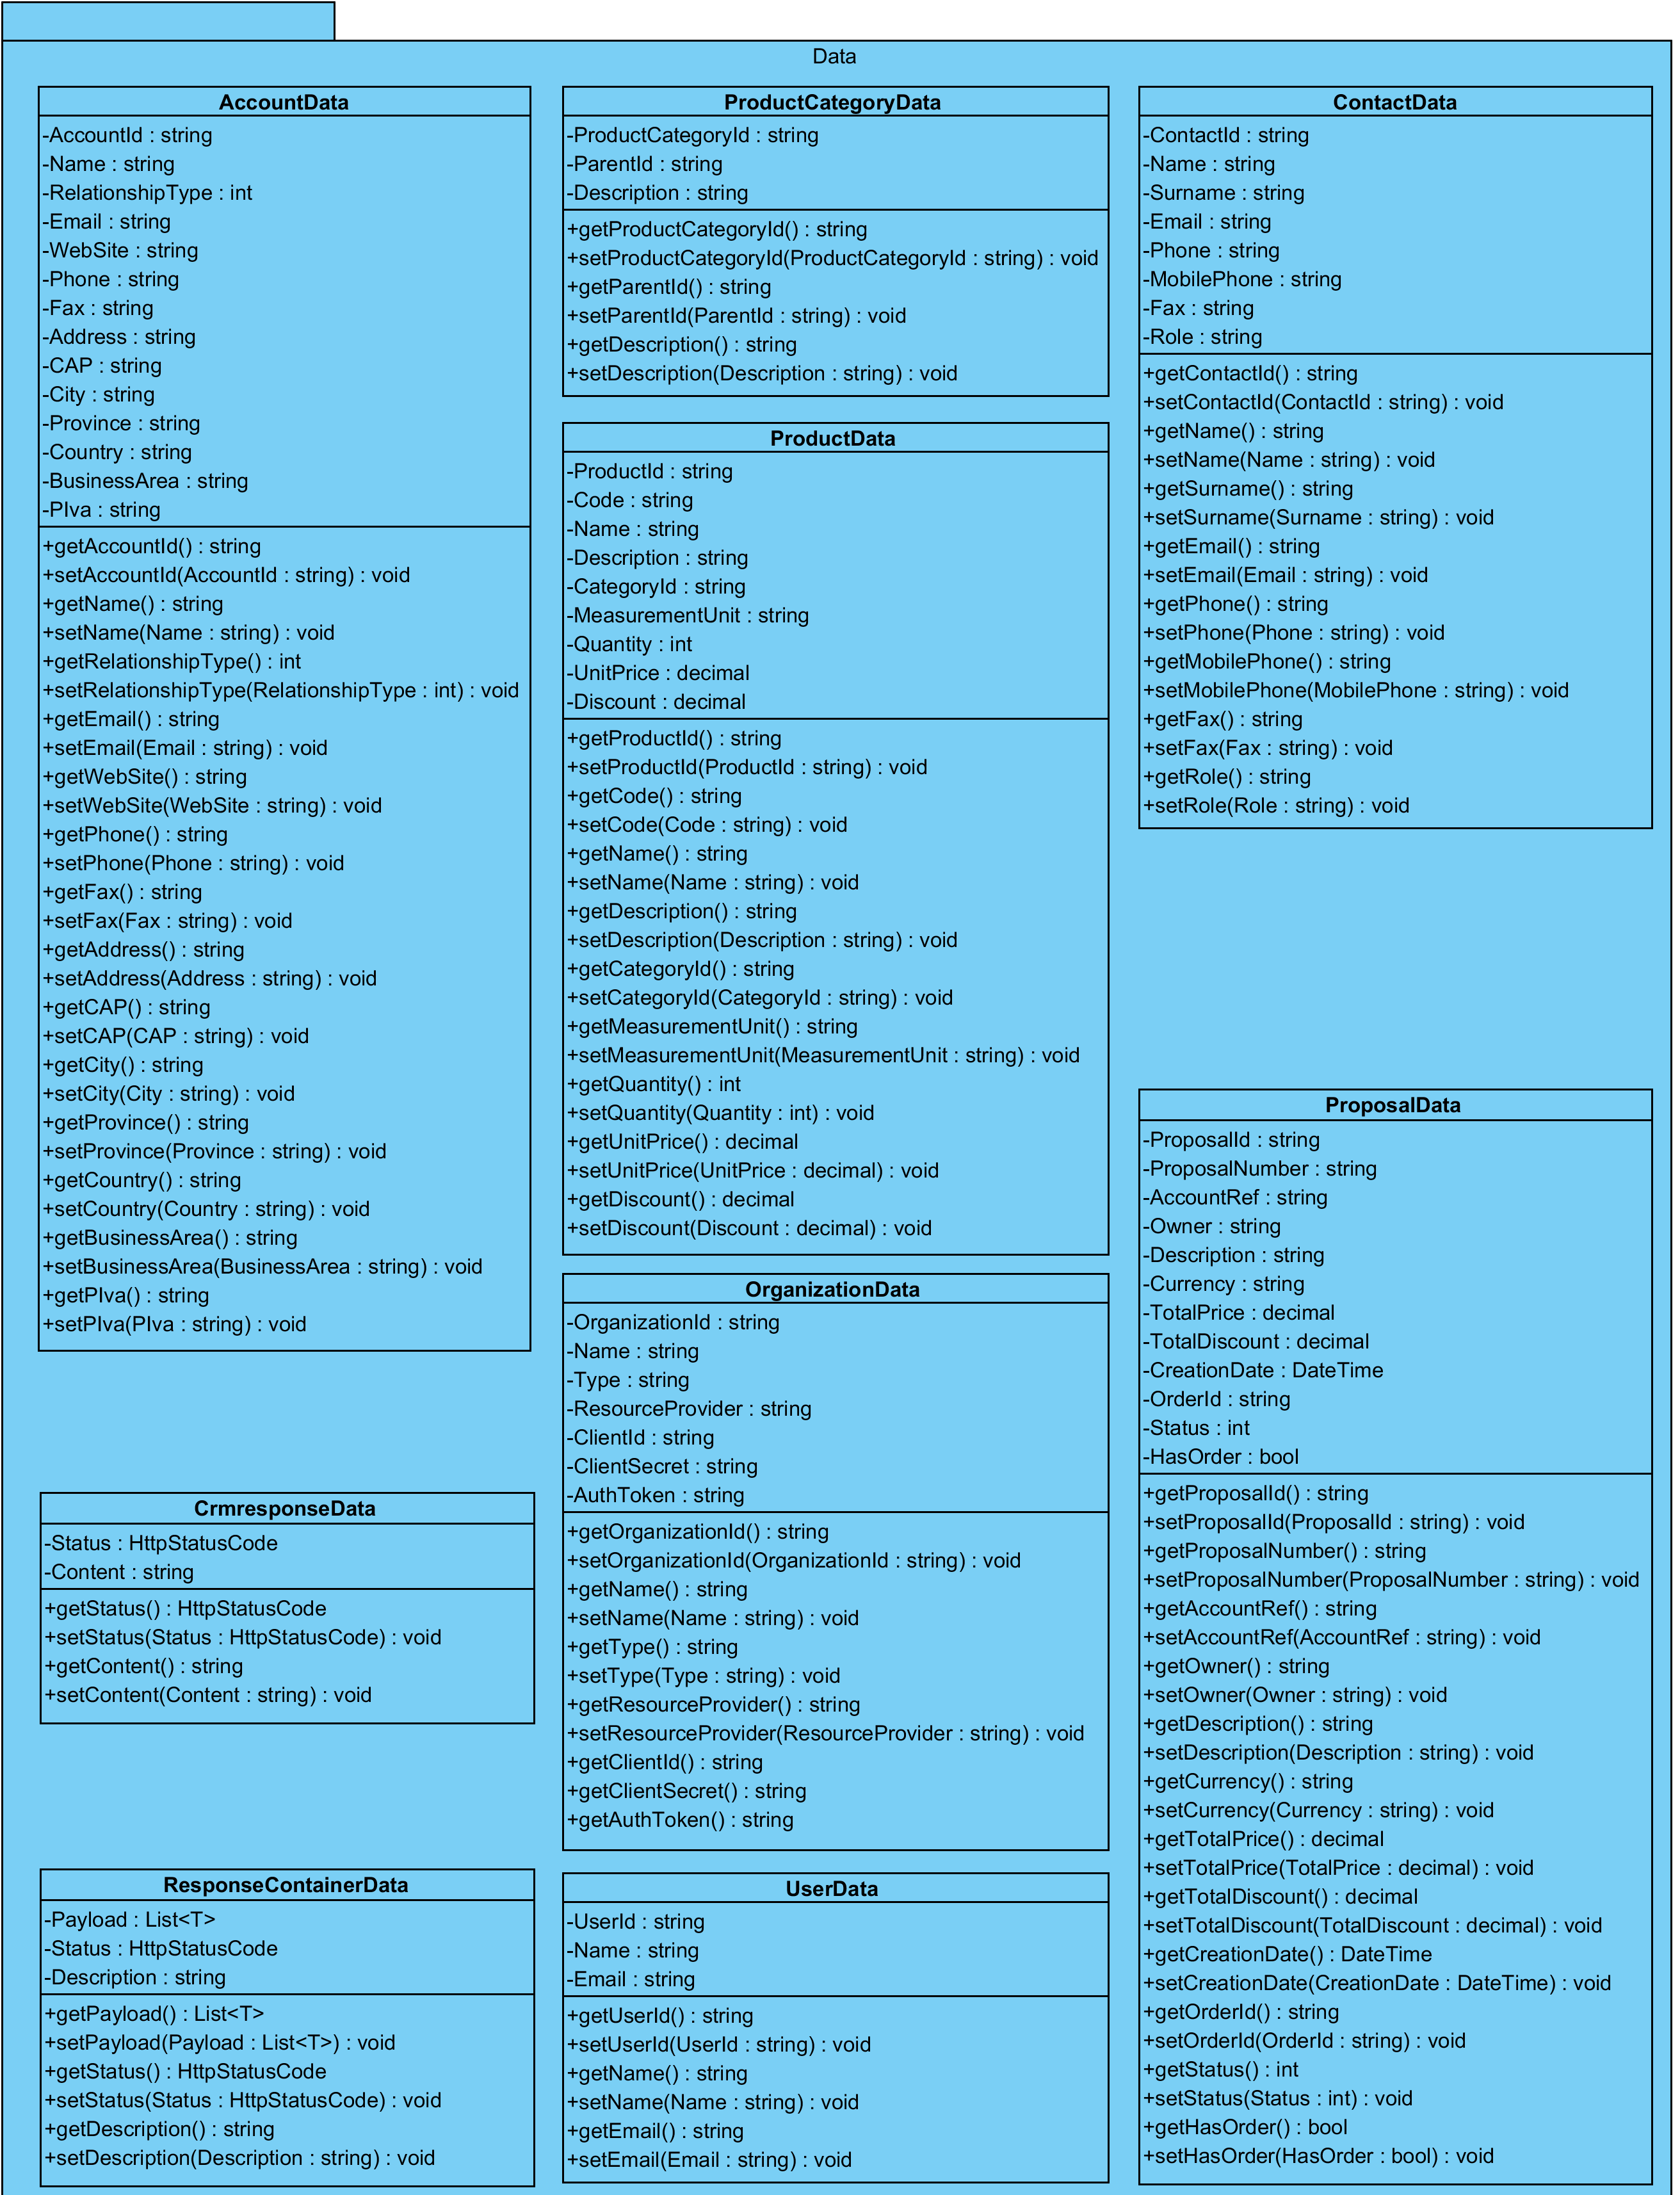
\includegraphics[width=\linewidth]{images/modules/Data}
	\caption{Diagramma UML del package Athesys.ADCrm.Common::Data}
	\label{fig:data}
\end{figure}

\paragraph{Description:}
Questo \glo{package} contiene tutti i vari \gls{DTO} definiti per ogni entità di dati che si vuole restituire alle chiamate effettuate da ADProject ed inoltre quelle necessarie per gestire le risposte le risposte provenienti dai CRM. 
Segue in questa sezione una breve descrizione delle classi principali, sorvolando sui metodi delle stesse in quanto sono tutti \glopl{accessor} \glo{getter} e \glo{setter}.


\subsubsection{ProposalData (class)}
\paragraph{Descrizione:}
Classe che rappresenta un oggetto \gls{DTO} per modellare l'entità \textit{Proposal}.
In essa sono presenti i metodi \glo{getter} e \glo{setter} e tutti i campi dati (privati) contenenti gli elementi che caratterizzano un offerta commerciale, quali: l'identificativo univoco della stessa, il cliente a cui è stata proposta, il costo totale, un eventuale sconto e molti altri dati.
Gli oggetti di questa classe, contenente i dati provenienti dal CRM, verranno incapsulati all'interno della risposta \gls{http} restituita ad ADProject.

\subsubsection{CrmResponseData (class)} \label{crmResponseDataClass}
\paragraph{Descrizione:}
Classe che rappresenta un oggetto \gls{DTO} per modellare le risposte \gls{http} provenienti dal \gls{CRM}.
Questa classe ha solamente due campi dati (ed i relativi \glopl{accessor}):
\begin{itemize}
	\item 	
	\begin{lstlisting}
	Private HttpStatusCode Status
	\end{lstlisting}
	In questo campo dati viene salvato il codice di stato \gls{http} della risposta mandata dal \gls{CRM};
	\item
	\begin{lstlisting}
	Private string Content
	\end{lstlisting}
	In questo campo dati viene salvato il \glo{JSON} della risposta mandata dal \gls{CRM}.
\end{itemize}

\subsubsection{ResponseContainerData (class)} \label{responseContainerDataClass}
\paragraph{Descrizione:}
Classe che rappresenta un oggetto \gls{DTO} per modellare le risposte \gls{http} da inviare a ADProject.
Questa classe ha tre campi dati (ed i relativi \glopl{accessor}):
\begin{itemize}
	\item 	
	\begin{lstlisting}
	private List<T> Payload
	\end{lstlisting}
	In questo campo dati è una lista di \glopl{generic} che viene istanziata al tipo di uno degli oggetti \gls{DTO} di questo \glo{package} (AccountData,ProposalData,ProductData,ContactData,UserData,ProductCategoryData o OrganizationData);
	
	\item 	
	\begin{lstlisting}
	private HttpStatusCode Status
	\end{lstlisting}
	In questo campo dati viene salvato il codice di stato \gls{http} che dovrà assumere la risposta da inviare ad ADProject;
	
	\item
	\begin{lstlisting}
	private string Description
	\end{lstlisting}
	In questo campo dati, in caso di errore, viene aggiunta una breve descrizione testuale dello stesso.
\end{itemize}




\subsection{Athesys.ADCrm.Model}
Questo \glo{package} contiene tutte le classi concrete in comune tra i \gls{CRM} che si vogliono collegare all'applicazione.
La classe principale del \glo{package} è Athesys.ADCrm.Model::Crm.
\subsubsection{Crm (class)} \label{crmClass}
\begin{figure}[H]
	\centering
	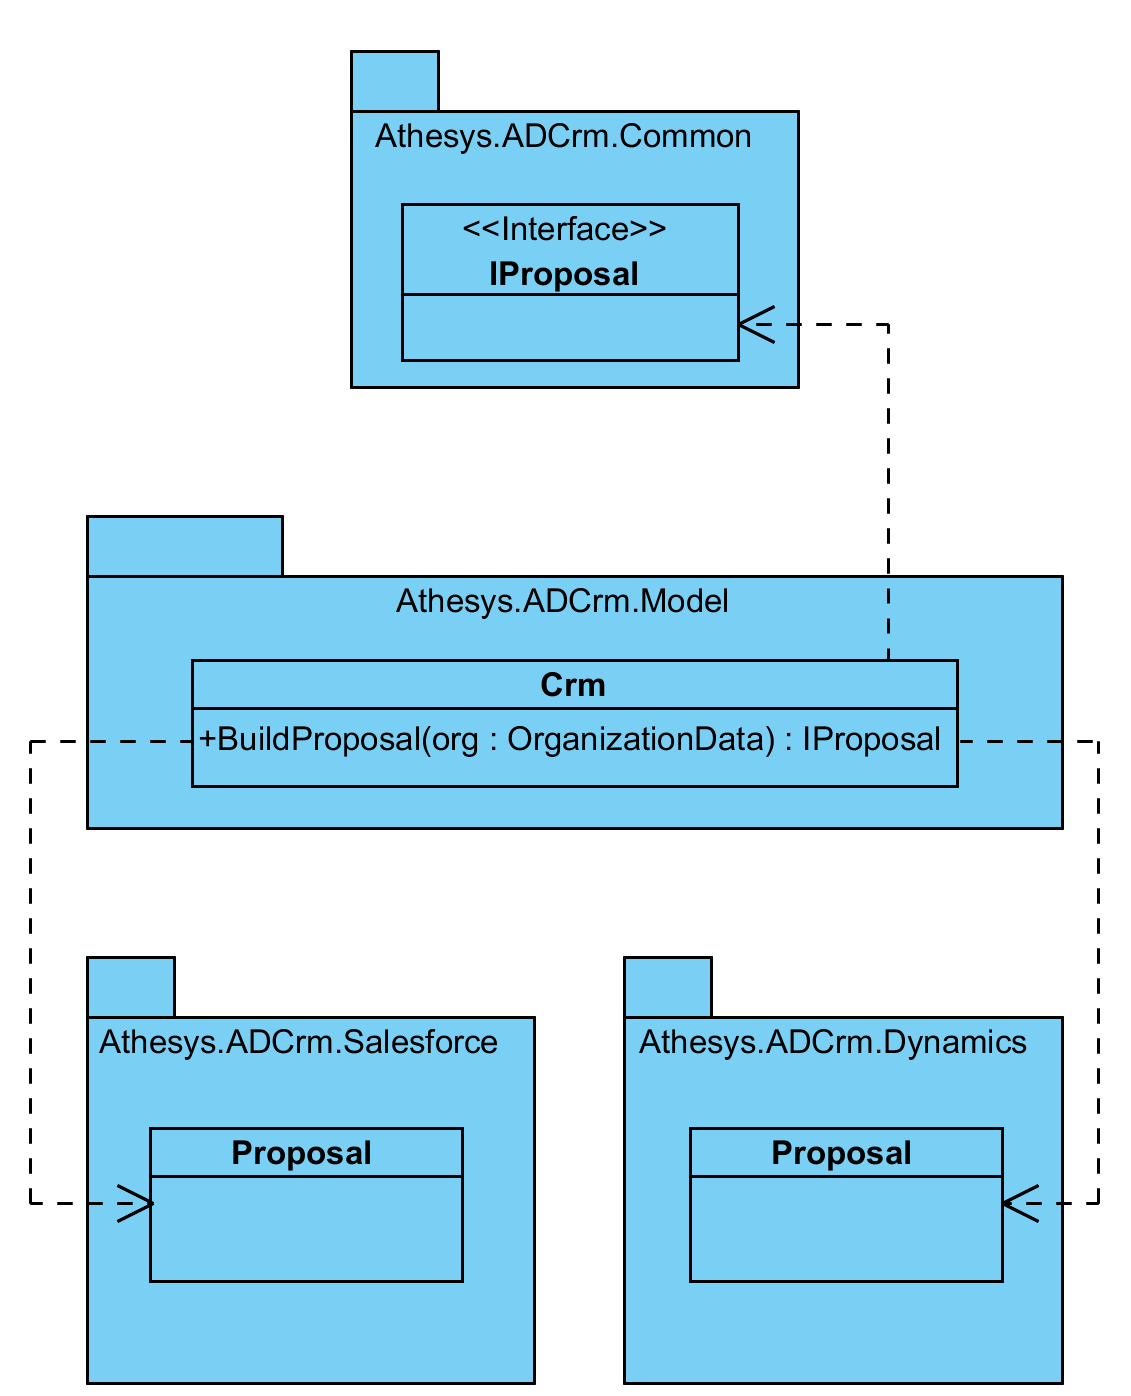
\includegraphics[width=\linewidth]{images/factoryInADCrm}
	\caption{Diagramma semplificato del pattern Factory per ADCrm}
	\label{fig:factoryInADCrm}
\end{figure}
\paragraph{Descrizione:}
Questa classe implementa il design pattern Factory ed è usata dai controllers per produrre oggetti concreti di un particolare \gls{CRM} (su cui invocare i metodi per recuperare i dati dallo stesso) senza conoscere a priori il tipo di \gls{CRM} richiesto (Dynamics o SalesForce).


Di seguito vengono riportati alcuni metodi significativi della classe per esemplificarne il funzionamento generale.


\paragraph{Metodi:}\hfill
\begin{itemize}
	\itemsep0em 
	\item 
	\begin{lstlisting}
	  public static async Task<OrganizationData> BuildOrganization(string organizationId)	
	\end{lstlisting}
	Metodo che costruisce un oggetto di tipo OrganizationData, appartenente ad un particolare \gls{CRM}, in base alla tipologia del parametro passato.
	Tutti i campi dati dell'oggetto ritornato vengono impostati dal database dell'applicazione che contiene i parametri di connessione ai vari \gls{CRM}.
	\\
	\textbf{\small Argomenti:}
	\begin{enumerate}[leftmargin=*]
		\itemsep0em 
		\item 
		\begin{lstlisting}
		organizationId : string
		\end{lstlisting}
		Rappresenta la tipologia di \gls{CRM} a cui ci si deve collegare. Questo dati si ottiene grazie alle route definite nella sezione \ref{apiRest} (eg. api/organization/\{\textbf{organizationId}\}/accounts).
	\end{enumerate}
	
	\item 
	\begin{lstlisting}
     public static IProposal BuildProposal(OrganizationData org)
	\end{lstlisting}
	Metodo che, in base alla tipologia di organizzazione passata per parametro, costruisce un oggetto Proposal per un particolare tipo di \gls{CRM}\\
	\textbf{\small Argomenti:}
	\begin{enumerate}[leftmargin=*]
		\itemsep0em
		\item 
		\begin{lstlisting}
		org : OrganizationData
		\end{lstlisting}
		Rappresenta la tipologia di \gls{CRM} da cui si vogliono recuperare le proposte commerciali.
	\end{enumerate}
\end{itemize}
 
\subsection{Athesys.ADCrm.Salesforce}\label{salesforce}
Questo \glo{package} contiene tutte le classi che implementano le interfacce definite in Athesys.ADCrm.Common e, sviluppando  restituiscono ai controllers di Athesys.ADCrm.API i vari oggetti \gls{DTO} delle entità del \glo{package} Athesys.ADCrm.Common.Data.
Di seguito vengono descritte brevemente le uniche tre classi che hanno un comportamento diverso da quanto sopracitato.

\subsubsection{ResponceMapper (class)}\label{responceMapperClass}
\paragraph{Descrizione:}
Questa classe ha la funzione di mappare le risposte provenienti dal \gls{CRM} modificandole in base alle esigenze di ADProject.
Per esempio se dal \gls{CRM} arrivasse una risposta d'errore con codice di stato \gls{http} 500 (quindi un errore interno del server), non si dovrà restituire ad ADProject una risposta lo stesso codice di stato, in quanto verrebbe interpretato come un errore del servizio e non del \gls{CRM}. C'è quindi l'esigenza di modificare ad-hoc le risposte per renderle fruibili dal richiedente delle stesse.
%TODO: controllare questa parte

\subsection{Athesys.ADCrm.Dynamics}\label{dynamics}
Questo \glo{package} contiene tutte le classi che implementano le interfacce definite in Athesys.ADCrm.Common e restituiscono ai controller di Athesys.ADCrm.API i vari oggetti \gls{DTO} di tipo Athesys.ADCrm.Common.Data al fine di incapsularli nella risposta \gls{http}.
Viene omessa la descrizione delle classi e dei metodi in quanto risulta identica a quella del \glo{package} \textit{Athesys.ADCrm.Salesforce}

\subsection{Database}
Il database è utilizzato per salvare i dati necessari a collegarsi per effettuare l'accesso e le richieste ai \gls{CRM}, vista la bassissima mole di dati da salvare si è deciso di optare per un semplicissimo database \glo{SQL} composto da una singola tabella, di nome Organization, avente la seguente struttura:
\begin{figure}[H]
	\centering
	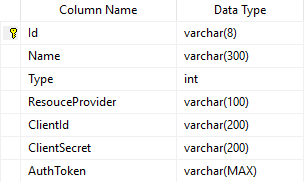
\includegraphics[width=0.7\linewidth]{images/schemaDB}
	\caption{Struttura tabella Organization del database}
	\label{fig:schemadb}
\end{figure}

\begin{itemize}
	\item \textbf{Id} : è un identificativo univoco alfanumerico, marcato come \textit{primary key} per poter distinguere i dati di  un'applicazione \gls{CRM} di una specifica azienda;
	\item \textbf{Name} : è il nome del software \gls{CRM} (eg. SalesForce o Dynamics);
	\item \textbf{Type} : è un campo intero per distinguere la tipologia di \gls{CRM} (eg. SalesForce o Dynamics)  
	\item \textbf{ResoureProvider} :
	Ogni software \gls{CRM} \textit{cloud-based} viene ospitato su un server, e per identificare a quale di questi ci si dovrà collegare, bisogna inserire questo campo nel \glo{url} (eg. \url{https://emea.salesforce.com} dove il campo ResoureProvider corrisponde alla voce \textit{emea} )
	%TODO: verificare il termine hostare
	\item \textbf{ClientId} : è l’identificativo univoco (pubblico) del client ed è uno dei dati fondamentali che le applicazioni \gls{CRM} devono fornire per permettere il collegamento di terze applicazioni-web tramite procedura OAuth;
	\item \textbf{ClietSecret} :  è l’identificativo segreto del client ed è il secondo dato fondamentale che le applicazioni \gls{CRM} devono fornire per permettere il collegamento di terze applicazioni-web tramite procedura OAuth;
	\item \textbf{AuthToken} : è il campo contenente la risposta \glo{JSON} restituita da un \gls{CRM} dopo la procedura di autenticazione OAuth; quindi non solo conterrà il \glo{token} da allegare per poter fare le richieste, ma anche il \glo{token} di refresh ed altri dati. Ne segue un esempio.
	
	
	\begin{lstlisting}[language=json,firstnumber=1]
	{
	"id":"https://login.salesforce.com/***",
	"issued_at":"1278448101416",
	"refresh_token":"***",
	"instance_url":"https://***.salesforce.com/",
	"signature":"***",
	"access_token":"***"
	}
	\end{lstlisting}
	
\end{itemize}


\subsection{Diagramma di sequenza}
	\begin{figure}[H]
	\centering
	\rotatebox{90}{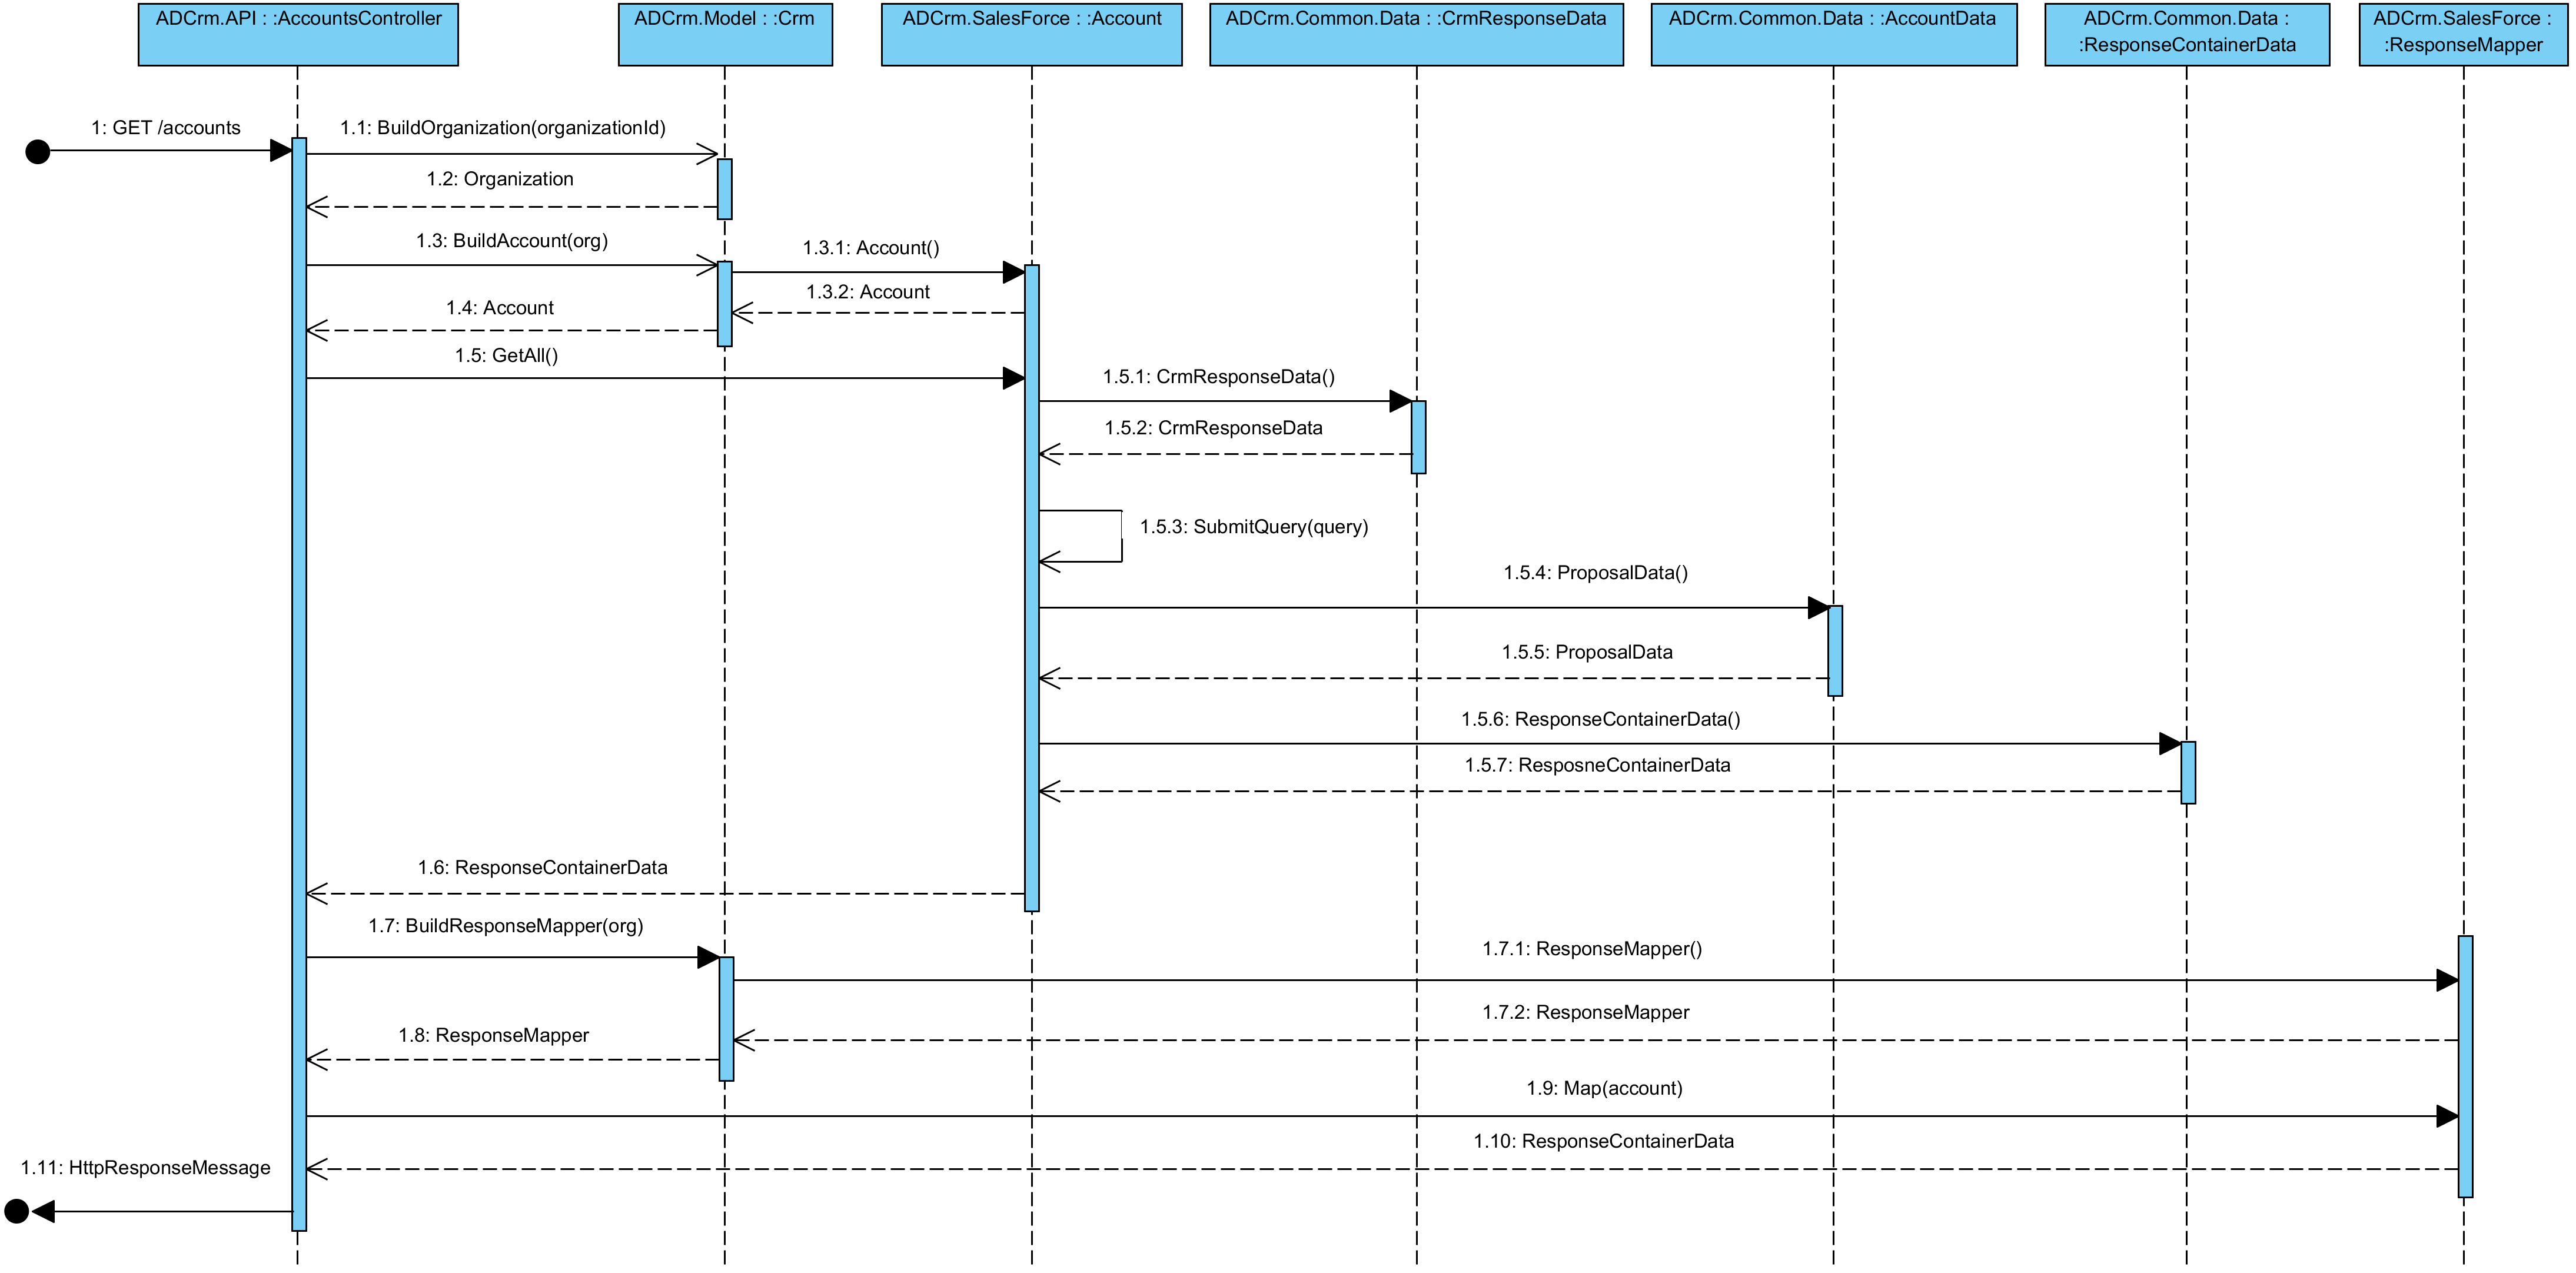
\includegraphics[width=.87\textheight,height=1.08\linewidth]{images/sdProposals}}
	
	\caption{Diagramma di sequenza per recuperare le entità Account da un \gls{CRM} }
	\label{fig:sdProposals}
\end{figure}

L'immagine soprastante è il diagramma di sequenza utile per facilitare la comprensione della catena di chiamate che viene effettuata per recuperare tutti i dati dei clienti dell'azienda dall'applicazione \gls{CRM} durante il lavoro in fase di codifica.

\begin{itemize}
	\item \textbf{AccountsController:} è l'oggetto che si occupa di invocare il metodo appropriato ogni volta che viene instradata una chiamata all'\glo{endpoint} "\textit{accounts}" (sez. \ref{accountsController});  
	\item \textbf{Crm:} è l'oggetto che implementa il design pattern \textit{Factory} (sez. \ref{factory}) costruendo oggetti per recuperare i dati da Salesforce o Dynamics (sez. \ref{crmClass});
	\item \textbf{Account:} è l'oggetto attraverso il quale vengono recuperati tutti i dati richiesti, riguardanti le aziende clienti, dal \gls{CRM};
	\item \textbf{CrmResponseData:} è un oggetto \gls{DTO} nel quale viene incapsulata la risposta \glo{JSON} restituita dal \gls{CRM} (sez. \ref{crmResponseDataClass});
	\item \textbf{AccountData:} è un oggetto \gls{DTO} che rappresenta l'account di un azienda cliente;
	\item \textbf{ResponseContainerData:}
	è un oggetto \gls{DTO} nel quale viene incapsulata la risposta \glo{JSON} che si restituirà all'applicazione chiamante, ADProject (sez. \ref{responseContainerDataClass});
	\item \textbf{ResponseMapper:} è la classe di utilità che si occupa di rimappare i codici \gls{http} delle risposte provenienti dal \gls{CRM} e di, in caso di errore modificare il JSON di risposta (sez. \ref{responceMapperClass}).

\end{itemize}